% 工程实践：以 Ubuntu 22.04 / ROS2 Humble 为主。
\subsubsection{先检查环境，再检查代码}
\label{sec:ros2-environment}

刚才节点已经跑起来了，不过你很快会遇到另一种问题：终端能运行，IDE 却说找不到包，或者明明改了源码，启动后还是昨天的输出。这时候先别急着改 C++，我们先看看程序到底用了哪套环境。系统安装称为底层工作空间（underlay），自己的安装目录称为覆盖工作空间（overlay）；先加载底层，再加载覆盖层，同名包就可能被后者覆盖。

\begin{center}
\begin{tabular}{p{0.40\textwidth}p{0.52\textwidth}}
\toprule[1.5pt]
变量 & 作用 \\
\midrule[1pt]
\nolinkurl{ROS_VERSION / ROS_DISTRO} & 判断当前终端所加载的 ROS 版本线索。\\
\texttt{AMENT\_PREFIX\_PATH} & ament 查找已安装包的前缀。\\
\texttt{CMAKE\_PREFIX\_PATH} & CMake 查找依赖的前缀。\\
\nolinkurl{PYTHONPATH / LD_LIBRARY_PATH} & Python 模块与动态库搜索路径。\\
\texttt{ROS\_DOMAIN\_ID} & 通信域编号；通信双方需要一致。\\
\texttt{ROS\_LOCALHOST\_ONLY} & DDS 实验中设为 1 时只与本机通信；Zenoh 的连接范围见后文配置。\\
\texttt{RMW\_IMPLEMENTATION} & 选择已经安装的中间件实现。\\
\bottomrule[1.5pt]
\end{tabular}
\end{center}

\begin{example}[确认终端实际使用的包]
完成前面的工作空间练习后，在新终端执行：
\par\medskip\noindent\begin{minipage}{\linewidth}
\begin{tbash}
source /opt/ros/humble/setup.bash
source ~/ros2_ws/install/setup.bash
printenv ROS_VERSION ROS_DISTRO AMENT_PREFIX_PATH
ros2 pkg prefix my_package
ros2 pkg executables my_package
\end{tbash}
\end{minipage}\par\smallskip
应显示 ROS 版本 2、发行版 humble，以及自己工作空间中的包安装前缀。若路径指向别的工作空间，先修正加载顺序；若找不到包，检查构建是否成功、包名是否一致。
\end{example}

\subsubsection{通信域与发现范围：只与自己的节点通信}
域编号用于把通信分组，不同域的节点之间不会互相通信。

\begin{example}[临时启用本机通信并恢复]
在两个终端分别执行下面的环境设置，然后分别运行 talker 与 listener。域 42 是这次练习的分组编号，实验室已有分配时换成你的编号：
\par\medskip\noindent\begin{minipage}{\linewidth}
\begin{tbash}
source /opt/ros/humble/setup.bash
export ROS_DOMAIN_ID=42
export ROS_LOCALHOST_ONLY=1
ros2 daemon stop
# 终端 A
ros2 run demo_nodes_cpp talker
# 终端 B
ros2 run demo_nodes_cpp listener
\end{tbash}
\end{minipage}\par\smallskip
应看到本机 listener 收到消息。在另一台机器使用相同域和普通网络发现时，无法收到本次本机发布的数据。

按 Ctrl+C 停止两个节点。在两个终端分别执行下列命令，再重新启动节点，恢复默认域和普通发现范围：
\par\medskip\noindent\begin{minipage}{\linewidth}
\begin{tbash}
unset ROS_LOCALHOST_ONLY ROS_DOMAIN_ID
ros2 daemon stop
\end{tbash}
\end{minipage}\par\smallskip
\end{example}

Humble 的本机实验使用 \texttt{export ROS\_LOCALHOST\_ONLY=1}。跨机器通信时，两端先取消本机限制，再设置相同域编号并重启节点与 daemon。

\begin{note}
建议大家调车时，记得设置只在本地通信。曾经学长在调试场地发现明明没启动自瞄的车居然还能收到图像消息，沉思了半个小时，差点要怀疑人生了，最后发现自己的手机非常的烫，才意识到是自己开了热点，所有车都在同一个域里互相通信了。
\end{note}

\paragraph*{用环境变量切换中间件}
\texttt{RMW\_IMPLEMENTATION} 用来选择已经安装的中间件实现。例如 Humble 默认的 Fast DDS 对应 \nolinkurl{rmw_fastrtps_cpp}。先停止旧节点，再在启动节点的两个终端分别设置：
\par\medskip\noindent\begin{minipage}{\linewidth}
\begin{tbash}
export RMW_IMPLEMENTATION=rmw_fastrtps_cpp
ros2 daemon stop
\end{tbash}
\end{minipage}\par\smallskip
重新启动节点后，新进程才会使用这个选择；用 \texttt{unset RMW\_IMPLEMENTATION} 可以恢复默认实现。安装其他实现后，改这个变量就能切换。具体安装、配置和对照实验留到第\ref{sec:ros2-rmw-selection}节，再结合大图像链路一起看。

\begin{conclusion}
\begin{itemize}
\item 找不到包：先确认构建、安装和环境加载，再修改代码。
\item 看不到节点：检查域、发现范围和 RMW，再检查 QoS 与接口。
\item 改了环境：重启相关节点与 daemon；变量只影响继承它的新进程。
\item 域与发现范围负责通信组织；认证和访问控制需要另行配置。
\end{itemize}
\end{conclusion}

\begin{exercise}
\label{ex:v2-ros-domain}
让本机 talker 使用域 42、listener 使用域 43，观察现象；把两端统一为 42 后重新启动并验证。写出恢复环境需要处理的进程和变量。
\end{exercise}

\Needspace{18\baselineskip}
\subsubsection{ament、colcon 与可复现的小工程}
\label{sec:ros2-ament}

到这里你已经接触了好几个名字：CMake、ament、colcon、rosdep。它们看起来都和“编译”有关，其实各自负责一段。我们下来详细介绍它们：CMake 描述单个 C++ 包怎样编译和安装，ament 提供 ROS2 的依赖、安装索引和导出约定，colcon 按依赖顺序构建工作空间中的多个包，rosdep 则根据依赖键安装系统依赖。

\begin{example}[建立共用教学包]
这次我们用一个简单心跳节点把依赖、测试、参数和启动文件串起来。源码在本卷 \path{examples/ros2/training_tools}，与前面的 my\_package 相互独立。先看看需要哪些文件：
\par\medskip\noindent\begin{minipage}{\linewidth}
\begin{lstlisting}[language={}]
training_tools/
  package.xml
  CMakeLists.txt
  src/heartbeat.cpp
  test/test_interval.cpp
  config/heartbeat.yaml
  launch/basic.launch.py
  launch/heartbeat.launch.py
  launch/team.launch.py
  launch/multi.launch.py
  launch/checked.launch.py
  cmake/Auto.cmake       # 只在自动宏实验时替换构建规则
\end{lstlisting}
\end{minipage}\par\smallskip
你可以把这个目录复制到 \path{~/ros2_ws/src}。也可以按下面逐个保存文件，先建目录：
\par\medskip\noindent\begin{minipage}{\linewidth}
\begin{tbash}
mkdir -p ~/ros2_ws/src/training_tools/{src,launch,config,test}
cd ~/ros2_ws/src/training_tools
\end{tbash}
\end{minipage}\par\smallskip
保存 \texttt{package.xml}。这份文件是依赖清单，里面写明了这个包的名字，版本，描述，维护者，许可证类型。不过这些对我们的实际使用都不是很重要，我们需要掌握的是里面具体写出依赖的部分，需要把这个包和其他包的依赖关系写清楚。否则在编译时可能导致先后顺序弄错而无法编译。\nolinkurl{<buildtool_depend>} 声明 ament 等构建工具，\nolinkurl{<build_depend>} 声明构建依赖，\nolinkurl{<build_export_depend>} 声明下游编译所需依赖，\nolinkurl{<exec_depend>} 声明运行依赖，\nolinkurl{<test_depend>} 声明测试依赖。\nolinkurl{<depend>} 合并普通依赖的构建、导出与运行三种用途。对于初学者而言，只要使用最后一个\nolinkurl{<depend>}就可以了。
\Needspace{23\baselineskip}
\par\medskip\noindent\begin{minipage}{\linewidth}
\lstinputlisting[frame=single,language=XML,caption={training\_tools/package.xml}]{examples/ros2/training_tools/package.xml}
\end{minipage}\par\smallskip
接下来保存 \nolinkurl{src/heartbeat.cpp}。构造函数读出 text 参数，创建发布者，再让定时器每 200 毫秒发一次消息。句柄保存在成员中；lambda 捕获 text 的值，所以参数只在启动时读取一次，改变文本实验时要重启节点。
\Needspace{35\baselineskip}
\par\medskip\noindent\begin{minipage}{\linewidth}
\lstinputlisting[frame=single,basicstyle=\ttfamily\footnotesize,language=C++,caption={heartbeat 的完整节点实现}]{examples/ros2/training_tools/src/heartbeat.cpp}
\end{minipage}\par\smallskip
然后保存 \texttt{CMakeLists.txt}。它找到清单里声明的依赖，编译 heartbeat，再安装程序和 Launch、YAML 资源。测试文件在下面提供，手工建包时先关闭测试，文件齐了再开启。
\par\medskip\noindent\begin{minipage}{\linewidth}
\lstinputlisting[frame=single,language=cmake,caption={手动声明依赖与安装规则}]{examples/ros2/training_tools/CMakeLists.txt}
\end{minipage}\par\smallskip
通用构建形式为 \texttt{colcon build [包选择选项] [构建选项]}：
\begin{center}
\begin{tabular}{p{0.42\textwidth}p{0.50\textwidth}}
\toprule[1.5pt]
参数 & 作用 \\
\midrule[1pt]
\texttt{--packages-select 包名} & 仅构建选定包，依赖需已可用。\\
\texttt{--packages-up-to 包名} & 构建目标及工作空间中的递归依赖。\\
\texttt{--symlink-install} & 在可用处采用符号链接安装。\\
\texttt{--cmake-args 参数} & 向 CMake 传递配置参数。\\
\bottomrule[1.5pt]
\end{tabular}
\end{center}
其余选项查询 \texttt{colcon build --help}。

一般来说，我们使用这条命令：
\par\medskip\noindent\begin{minipage}{\linewidth}
\begin{tbash}
colcon build --symlink-install --cmake-args -DCMAKE_BUILD_TYPE=Release
\end{tbash}
\end{minipage}\par\smallskip
它会构建工作空间中所有包，并在可用处使用符号链接。使得我们修改参数时不必重新编译。Release 模式优化编译速度和运行效率。为了方便起见，我们可以在 \texttt{~/.bashrc} 或 \texttt{~/.zshrc} 中写一个别名：
\par\medskip\noindent\begin{minipage}{\linewidth}
\begin{tbash}
alias cb='colcon build --symlink-install --cmake-args -DCMAKE_BUILD_TYPE=Release'
\end{tbash}
\end{minipage}\par\smallskip

下面先关闭测试，把节点跑通。rosdep 第一次使用时需初始化：系统尚无默认源列表时执行一次 \texttt{sudo rosdep init}，然后用普通用户执行 \texttt{rosdep update}；已经初始化就跳过 init。接下来让它从清单中安装缺少的依赖：
\par\medskip\noindent\begin{minipage}{\linewidth}
\begin{tbash}
cd ~/ros2_ws
source /opt/ros/humble/setup.bash
rosdep install --from-paths src --ignore-src -r -y
colcon build --packages-select training_tools --cmake-args -DBUILD_TESTING=OFF
source install/setup.bash
ros2 run training_tools heartbeat
\end{tbash}
\end{minipage}\par\smallskip
另一终端加载相同环境后运行 \texttt{ros2 topic echo /status}，应持续收到 ready。消息发布约 5 Hz。
\end{example}

\Needspace{18\baselineskip}
\subsubsection{自动依赖、库导出与构建测试}
也许你已经觉得CMake里面的内容实在是冗长，每个包都需要 \nolinkurl{find_package}，然后\nolinkurl{target_link_libraries}，这样写一大串。
别担心， \texttt{ament\_cmake\_auto} 可以轻松地帮你减少重复声明。
它依据清单寻找依赖。
注意第三方库的 rosdep 键与 CMake 名称可能不同，例如OpenCV通过 \verb|rosdep resolve opencv2| 查询依赖，而 CMake  需要使用 \verb|find_package(OpenCV REQUIRED)|。这种时候Cmake里面的 \verb|find_package| 还是需要手动写的。

\begin{example}[同一个包改用 ament 自动宏]
在 \texttt{package.xml} 中把构建工具依赖改为 \texttt{ament\_cmake\_auto}，保留 export 中的 \texttt{ament\_cmake} 构建类型。把本项目 \path{cmake/Auto.cmake} 的内容复制为包根目录的 CMakeLists.txt，完整规则如下：
\par\medskip\noindent\begin{minipage}{\linewidth}
\lstinputlisting[frame=single,language=cmake,caption={自动宏构建规则}]{examples/ros2/training_tools/cmake/Auto.cmake}
\end{minipage}\par\smallskip
重新执行 rosdep 安装和前例的构建、运行命令，行为应相同。下来大家在写自己的ROS包时，手动版本和自动版本二选一即可。
\end{example}

若包要供其他包链接，还需安装库和公开头文件。手动构建时，用 \nolinkurl{ament_export_targets} 导出目标，用 \nolinkurl{ament_export_dependencies} 导出依赖；自动宏可简化这些规则。

文件末尾调用 \nolinkurl{ament_package()}，自动版本则调用 \nolinkurl{ament_auto_package()}，完成包索引与配置生成。

组件化还需要代码中的 \nolinkurl{RCLCPP_COMPONENTS_REGISTER_NODE} 和 CMake 的 \nolinkurl{rclcpp_components_register_nodes} 注册。这些我们会在第\ref{sec:ros2-image-components}节会用完整的图像工程，把组件注册、Launch 布局与数据所有权接起来。

\begin{example}[把参数边界变成自动检查]
在 \nolinkurl{test/test_interval.cpp} 保存一个无硬件依赖的边界测试。
\Needspace{20\baselineskip}
\par\medskip\noindent\begin{minipage}{\linewidth}
\lstinputlisting[frame=single,language=C++,caption={独立的间隔边界测试}]{examples/ros2/training_tools/test/test_interval.cpp}
\end{minipage}\par\smallskip
在工作空间根目录执行：
\par\medskip\noindent\begin{minipage}{\linewidth}
\begin{tbash}
colcon build --packages-select training_tools --cmake-args -DBUILD_TESTING=ON
colcon test --packages-select training_tools
colcon test-result --verbose
\end{tbash}
\end{minipage}\par\smallskip
两组测试应通过。更多测试规则请查阅 \href{https://google.github.io/googletest/}{GTest官方文档}。
\end{example}

\begin{conclusion}
\begin{itemize}
\item 清单声明依赖；rosdep 安装系统依赖；CMake/ament 使用它们构建包。
\item colcon 组织多个包，安装后的索引让 ROS2 能查到可执行程序和资源。
\item 库的导出影响下游使用；只在本包编译成功还不够。
\item 自动宏减少重复配置。
\end{itemize}
\end{conclusion}
\begin{exercise}
\label{ex:v2-ros-ament}
说明为什么源目录已有 launch 文件，\texttt{ros2 launch} 仍可能找不到它。将上例合法间隔上限改为 500，同时修改边界测试并重新验证。
\end{exercise}

\section{Launch 启动配置与模块组合}
\subsubsection{Launch 入门：用一个文件启动节点}
\label{sec:ros2-launch}

你现在已经能手动启动节点了。不过真正上车时，相机、识别、串口各开一个终端，每个节点后面再跟一串参数，少打一个字，机器人就可能和你玩捉迷藏。启动文件（launch file）把这次需要运行的程序和配置记下来，下次用一条命令就能把它们重新启动。我们先让刚才的 heartbeat 跑起来，再逐步加上参数、命名空间和组合启动，最后看看需要按条件、按事件启动时怎么写。

ROS2 支持 Python、XML 和 YAML 格式的启动文件。本节使用 Python：基础配置可以直接写，后面需要循环、检查文件或处理事件时，也能沿着同一种写法继续扩展。启动文件用什么语言，和节点用什么语言没有关系；Python Launch 完全可以启动我们刚写好的 C++ 节点。

\paragraph*{先写一个只启动节点的文件}
Python 启动文件的入口是 \nolinkurl{generate_launch_description()}。ROS2 加载文件后会调用它，得到一个 \texttt{LaunchDescription}，也就是这次启动要执行的动作列表。动作（action）不一定是节点，还可以是设置环境、引入另一个启动文件或注册事件处理器。\texttt{Node} 来自 \texttt{launch\_ros}，是在通用启动系统之上增加了 ROS 节点配置的动作。

\begin{example}[把 ros2 run 写进启动文件]
继续使用前面的 training\_tools，不需要新建包。在包内保存 \nolinkurl{launch/basic.launch.py}，完整文件如下：
\par\medskip\noindent\begin{minipage}{\linewidth}
\lstinputlisting[frame=single,language=Python,caption={先启动一个心跳节点}]{examples/ros2/training_tools/launch/basic.launch.py}
\end{minipage}\par\smallskip
这里的 \texttt{package} 是功能包名，\texttt{executable} 是安装后的可执行程序名。它们对应 \texttt{ros2 run training\_tools heartbeat} 中的两个名字。\texttt{name} 覆盖节点在源码里设置的名字，程序名不变，节点名可以按启动需要另取。\texttt{output='screen'} 让子进程的输出显示在当前终端。

通用启动形式为 \texttt{ros2 launch 包名 文件名 [参数名:=值]}。前面的 CMake 已经安装整个 launch 和 config 目录，不过新增文件后仍要重新构建，让安装目录也有它。下面的命令在工作空间根目录执行：
\par\medskip\noindent\begin{minipage}{\linewidth}
\begin{tbash}
cd ~/ros2_ws
source /opt/ros/humble/setup.bash
colcon build --packages-select training_tools
source install/setup.bash
ros2 launch training_tools basic.launch.py
\end{tbash}
\end{minipage}\par\smallskip
另开一个终端，加载相同的底层和覆盖工作空间后检查：
\par\medskip\noindent\begin{minipage}{\linewidth}
\begin{tbash}
ros2 node list
ros2 topic echo /status std_msgs/msg/String --once
\end{tbash}
\end{minipage}\par\smallskip
你应能找到 \texttt{/heartbeat}，并收到一条 ready。回到启动终端按 Ctrl+C，Launch 会通知它管理的进程退出，再也不用逐个终端关节点了。
\end{example}

写 \texttt{Node(...)} 时，我们只是在描述“等会儿怎样启动”，并没有当场执行程序。把它放进返回的动作列表，启动系统才会处理它。这个区别后面会解释为什么参数不能直接当 Python 字符串用，也会解释为什么“写在前面”不等于“已经准备好了”。

\Needspace{18\baselineskip}
\subsubsection{Launch 配置：名字、YAML 与命令行参数}
刚才只有四个字段。真正开始连模块时，常用配置还包括下面这些：
\begin{center}
\begin{tabular}{p{0.25\textwidth}p{0.67\textwidth}}
\toprule[1.5pt]
字段 & 本节怎样使用 \\
\midrule[1pt]
\texttt{package / executable} & 找到已经安装的程序。\\
\texttt{name / namespace} & 设置节点名与命名空间，例如 \nolinkurl{/red/heartbeat}。\\
\texttt{parameters} & 传入参数字典、ROS 参数 YAML 文件，或把两者组合起来。\\
\texttt{remappings} & 用 \texttt{(原名, 新名)} 修改话题、服务等接口名称。\\
\texttt{output} & 设置子进程输出的去向；本节用 screen，日志出口见第\ref{sec:ros2-logging}节。\\
\texttt{additional\_env} & 在继承的环境上为这个进程增补环境变量。\\
\bottomrule[1.5pt]
\end{tabular}
\end{center}

先把三个“名字”分开：包名帮助 ROS2 找程序，节点名帮助你在计算图里找节点，话题名决定数据从哪里进、从哪里出。改节点名不会把它发布的所有话题一并改名。比如 heartbeat 源码里发布的是相对话题 \texttt{status}；加上 \texttt{namespace='red'}，完整名字就变成 \texttt{/red/status}。再写 \texttt{remappings=[('status', 'health')]}，最终发布到 \texttt{/red/health}。

这里的相对名字会跟着命名空间走，而以 \texttt{/} 开头的绝对名字从根开始。例如把重映射目标写成 \texttt{/health}，结果就是 \texttt{/health}，不会再加 red。相机驱动发布 image\_raw，识别节点订阅 image，也可以通过重映射把它们接到同一个名字。不过你要分别核对两端的最终话题、类型和 QoS，Launch 不会替你修好接口不匹配的问题。

\paragraph*{先放进 YAML，再把常改的值留给命令行}
配置还少的时候，直接写 \texttt{parameters=[\{'text': 'ready'\}]} 就够用了。配置多起来之后，把它们放进 YAML 更方便比较和保存；经常随机器人或实验变化的几项，再通过启动参数（launch argument）从命令行传入。我们把这两种办法放在同一个例子里。

\begin{example}[保存配置，并在启动时覆盖它]
在 training\_tools 包内保存 \nolinkurl{config/heartbeat.yaml}：
\par\medskip\noindent\begin{minipage}{\linewidth}
\lstinputlisting[frame=single,language={},caption={心跳节点的 ROS 参数文件}]{examples/ros2/training_tools/config/heartbeat.yaml}
\end{minipage}\par\smallskip
\texttt{ros\_\_parameters} 下面才是节点参数。最外层的 \texttt{/**} 是通配节点键，让这份简单配置在节点改名或加命名空间后仍适用。若只想配置 \nolinkurl{/red/heartbeat}，也可以把这个键改成它的完整名字；名字不匹配时，文件虽然找到了，参数却不会落到你想配置的节点上。多节点系统也要留意通配键的范围，别把本来只给一个节点的配置发给其他节点。

接下来保存 \nolinkurl{launch/heartbeat.launch.py}。这次让 robot 控制命名空间，text 控制消息内容，params\_file 控制 YAML 路径：
\par\medskip\noindent\begin{minipage}{\linewidth}
\lstinputlisting[frame=single,basicstyle=\ttfamily\footnotesize,language=Python,caption={可从命令行配置的心跳启动文件}]{examples/ros2/training_tools/launch/heartbeat.launch.py}
\end{minipage}\par\smallskip

我们按使用顺序拆开看。\nolinkurl{get_package_share_directory('training_tools')} 从安装索引找到这个包的资源目录，\texttt{Path} 再把 config 和文件名接上。这样把工作空间搬到另一台机器，启动文件仍能找到随包安装的配置；不必把自己的 \path{/home/student/ros2_ws/src/...} 写死在里面。

\nolinkurl{DeclareLaunchArgument} 声明启动参数，给出默认值和说明。\nolinkurl{LaunchConfiguration('robot')} 则表示“执行到这里时，取 robot 的实际值”。它是一个替换对象（substitution），不是已经取出的 Python 字符串。声明参数不会自动修改节点：robot 必须接到 namespace 上，text 必须接到 parameters 上，它们才会影响这次运行。

\texttt{parameters} 中先放 YAML 路径，再放一个字典，后面的 text 会覆盖 YAML 中的同名项。因此，只运行这个文件而不传 text，收到的是默认启动参数 \texttt{ready from launch}，不是 YAML 中的 \texttt{ready from yaml}。这很适合“文件保存基础配置，命令行改少数常用项”的做法；如果你希望完全采用 YAML 的 text，就删除后面的 text 字典，让文件决定它。

最后，\texttt{ParameterValue(..., value\_type=str)} 明确告诉 Launch：text 要作为字符串传入。命令行传来的是文本，但 ROS 参数求值时可能把 true、123 这类内容解释成布尔量或整数，而 heartbeat 声明的 text 是字符串。把类型写清楚，可以避免“明明传了字，怎么说类型不对”的疑惑，真正的整数或布尔参数也可以相应指定 \texttt{int} 或 \texttt{bool}。

重新构建并加载环境后，先看这个文件允许传什么，再启动：
\par\medskip\noindent\begin{minipage}{\linewidth}
\begin{tbash}
ros2 launch training_tools heartbeat.launch.py --show-args
ros2 launch training_tools heartbeat.launch.py robot:=red text:=tracking
\end{tbash}
\end{minipage}\par\smallskip
\texttt{--show-args} 显示参数说明后退出，不会启动节点。第二条命令会启动 \nolinkurl{/red/heartbeat}，在另一终端检查：
\par\medskip\noindent\begin{minipage}{\linewidth}
\begin{tbash}
ros2 topic echo /red/health std_msgs/msg/String --once
ros2 param get /red/heartbeat text
ros2 node info /red/heartbeat
\end{tbash}
\end{minipage}\par\smallskip
应收到 tracking，参数查询也应显示 tracking，节点信息中能找到 \texttt{/red/health}。如果内容包含空格，把整个赋值参数加引号，例如 \texttt{'text:=ready for battle'}。若要使用另一份 YAML，传 \texttt{params\_file:=/实际路径/参数.yaml}。
\end{example}

\begin{note}
启动参数属于 Launch，节点参数属于运行中的 ROS 节点。\texttt{ros2 param get /red/heartbeat robot} 查不到本例的 robot，因为它只用来选择命名空间，并没有作为节点参数传入。\texttt{use\_sim\_time} 则是常见节点参数：需要模拟时钟的节点应一致设置，并有 \texttt{/clock} 来源；只给 Launch 声明一个同名参数不会自动配置所有节点。我们的 heartbeat 使用 \nolinkurl{create_wall_timer}，发布周期也不会因为设置模拟时间就自动改成模拟时钟。
\end{note}

\begin{exercise}
\label{ex:v2-ros-launch-basic}
把 basic 文件的节点名改为 pulse，确认程序仍叫 heartbeat、话题仍是 \texttt{/status}。然后用 heartbeat 启动文件传入 \texttt{robot:=blue text:=true}，查询完整节点名、最终话题名和 text 的参数类型。最后只在你的练习副本中删除覆盖 text 的字典，重新启动，说明消息为什么变回 YAML 中的内容。
\end{exercise}

\subsubsection{Launch 组合：引入子文件与条件启动}
现在 heartbeat 已经能独立启动了。系统里再加一个观测程序时，我们没必要在新的launch文件中复制刚才的配置，而是可以用 \nolinkurl{IncludeLaunchDescription} 引入它。相机、识别、串口以后也可以各保留一个启动文件，最外层的 bringup 文件只负责把它们组合起来。需要改相机参数时，就不用在一份几百行的文件里翻半天。

\begin{example}[按条件观测一条消息]
保存 \nolinkurl{launch/team.launch.py}。本例用 \texttt{ExecuteProcess} 启动 \texttt{ros2 topic echo}，它是一个普通命令行进程；启动 ROS 节点通常仍用 \texttt{Node}，这样不必自己拼接 ROS 参数。完整文件如下：
先导入需要的工具，并定义打印配置的辅助函数：
\par\medskip\noindent\begin{minipage}{\linewidth}
\lstinputlisting[frame=single,basicstyle=\ttfamily\footnotesize,language=Python,firstline=1,lastline=18,caption={team 的导入与辅助函数}]{examples/ros2/training_tools/launch/team.launch.py}
\end{minipage}\par\smallskip

接着在同一个文件里写出完整入口，把这些动作组合起来：
\par\medskip\noindent\begin{minipage}{\linewidth}
\lstinputlisting[frame=single,basicstyle=\ttfamily\footnotesize,language=Python,firstline=19,caption={team 的完整启动入口}]{examples/ros2/training_tools/launch/team.launch.py}
\end{minipage}\par\smallskip

入口函数里，我们先安排引入部分。目标文件交给 \nolinkurl{PythonLaunchDescriptionSource}，说明它是 Python 启动文件；\texttt{launch\_arguments} 把主文件的配置传给子文件。这里需要的是键值对序列，所以字典最后调用 \texttt{.items()}。主文件的 robot 接到了子文件的 robot，子文件再把它接到节点命名空间；text 固定传为 \texttt{team ready}，因此覆盖子文件的默认启动值。

再看观测开关：\nolinkurl{IfCondition(LaunchConfiguration('watch'))} 在 watch 为 true 或 1 时执行这个动作，为 false 或 0 时跳过；\texttt{UnlessCondition} 正好反过来，所以关闭观测时会打印 \texttt{Observer disabled.}。布尔值不区分大小写，其他写法可能报错。不要写 Python 的 \nolinkurl{if LaunchConfiguration('watch'):}，也不要用 \texttt{bool('false')}：前者检查的是一个 Python 对象，后者仍为真，都没有按启动参数的布尔含义判断。

入口里还设置了环境。\nolinkurl{SetEnvironmentVariable} 在所在 Launch 上下文中设置变量，影响之后使用这份环境启动的进程。本例的这个环境变量会把控制台颜色打开，这里仅做演示，实际工作中推荐大家把这个环境变量直接设置到\path{~/.bashrc}中保持终端的可读性。只给一个节点加变量时，用 heartbeat 文件中的 \texttt{additional\_env} 更直接，它会保留原有 PATH、库搜索路径等配置。\texttt{env} 则用于从一份完整环境开始设置，不适合只想补一个变量的情况。Launch 改动的是它管理的环境，不会反过来修改已经打开的父终端。

重新构建、加载环境，然后分别运行：
\par\medskip\noindent\begin{minipage}{\linewidth}
\begin{tbash}
ros2 launch training_tools team.launch.py
ros2 launch training_tools team.launch.py watch:=false
\end{tbash}
\end{minipage}\par\smallskip
第一轮收到一条 team ready 后，观测进程退出，heartbeat 继续运行；第二轮只启动 heartbeat，并打印关闭观测的提示。这里的观测话题故意固定为 \texttt{/red/health}，所以先保留 robot 的默认值。只改 \texttt{robot:=blue} 时，发布者去了 blue，观测者却还在等 red；下面的练习会让它们一起跟着配置变化。至于 \texttt{OpaqueFunction} 和退出提示，我们稍后再拆开解释。
\end{example}

\begin{exercise}
\label{ex:v2-ros-launch}
将 team 启动文件的观测话题也与 robot 参数绑定，以 \texttt{robot:=blue} 启动，确认一次性观测能退出。再用 \texttt{watch:=false} 确认只启动 heartbeat，并出现关闭观测的提示。说明主文件的 robot、子文件的 robot 和节点命名空间是怎样接起来的。
\end{exercise}

\subsubsection{Launch 分组：命名空间与多实例启动}
如果红、蓝两套传感器都要启动同一种程序，只给它们改节点名还不够，话题也要分开。\nolinkurl{GroupAction} 可以把一组动作放在同一个作用域里；默认的 \texttt{scoped=True} 会在离开组时恢复启动配置和环境，\texttt{PushRosNamespace} 也会随这个组退出而恢复。这样给 red 加的命名空间就不会跑到后面的 blue 身上。

\begin{example}[复用同一份启动文件，得到两套独立话题]
保存 \nolinkurl{launch/multi.launch.py}：
\par\medskip\noindent\begin{minipage}{\linewidth}
\lstinputlisting[frame=single,basicstyle=\ttfamily\footnotesize,language=Python,caption={分组启动红蓝两套心跳}]{examples/ros2/training_tools/launch/multi.launch.py}
\end{minipage}\par\smallskip

这里的 Python 循环只是生成两组动作，每组都有自己新建的 Include 动作。\nolinkurl{PushRosNamespace('red')} 先加外层命名空间，子文件又通过 robot 得到相对命名空间 sensors，两者接成 \texttt{/red/sensors}。blue 那组则得到 \texttt{/blue/sensors}。参数名 robot 只是我们取的名字，并不会自动推断哪一段代表机器人；你传进去什么，子文件就使用什么。

重新构建、加载环境后启动，并在另一终端查询：
\par\medskip\noindent\begin{minipage}{\linewidth}
\begin{tbash}
# 启动终端
ros2 launch training_tools multi.launch.py
# 查询终端，先加载相同环境
ros2 node list
ros2 topic echo /red/sensors/health std_msgs/msg/String --once
ros2 topic echo /blue/sensors/health std_msgs/msg/String --once
\end{tbash}
\end{minipage}\par\smallskip
两条话题应分别返回 red ready 和 blue ready，对应节点是 \nolinkurl{/red/sensors/heartbeat} 与 \nolinkurl{/blue/sensors/heartbeat}。因为节点和重映射都使用相对名字，整个模块才能跟着外层命名空间走；如果子文件把名字写成 \texttt{/health}，两套模块就又挤到同一条绝对话题上了。
\end{example}

\begin{exercise}
\label{ex:v2-ros-launch-group}
在 multi 的练习副本里增加 green，把子文件的相对命名空间 sensors 改为 camera。先写出三个节点和三个发布话题的完整名字，再运行核对。若把子文件 remappings 的目标改成 \texttt{/health}，三个发布者会落在哪里？说明为什么分组不能自动隔离绝对话题名。
\end{exercise}

\subsubsection{Launch 事件：进程状态与模块就绪}
回头看 team 中的 \nolinkurl{RegisterEventHandler}。它注册了一个 \texttt{OnProcessExit} 处理器，\nolinkurl{target_action=observer} 指向前面创建的那个观测动作；观测进程退出时，启动系统再执行 \texttt{on\_exit} 列表里的 \texttt{LogInfo}。这里传的是动作对象，不是节点名字，也不是把同样参数再写一遍创建的新对象。处理器放在目标动作之前注册，可以避免错过很快启动、很快退出的进程。

常见事件先记住下面几种，真要用时再查完整接口：
\begin{center}
\begin{tabular}{p{0.31\textwidth}p{0.61\textwidth}}
\toprule[1.5pt]
处理器 & 它观察到的事情 \\
\midrule[1pt]
\texttt{OnProcessStart} & 目标进程已经启动，可记录进程启动或执行后续动作。\\
\texttt{OnProcessExit} & 目标进程已经退出；正常结束和异常退出都可能触发。\\
\texttt{OnProcessIO} & 进程产生了标准输出或标准错误，可处理这些输出。\\
\texttt{OnShutdown} & Launch 收到了关闭事件，例如用户按下 Ctrl+C。\\
\bottomrule[1.5pt]
\end{tabular}
\end{center}

\texttt{on\_exit} 里还可以放新的启动动作，或者用 \texttt{EmitEvent(event=Shutdown(reason='...'))} 请求关闭整套 Launch。比如相机进程退出后，你希望一起结束依赖它的识别进程，就可以为相机注册退出处理器。若只有正常退出才继续下一步，应在回调中检查事件的 \texttt{returncode}。本例只打印提示，所以观测退出不会结束心跳。

不过，\nolinkurl{LaunchDescription([node_a, node_b])} 并不保证 A 完成初始化后才启动 B；\texttt{OnProcessStart} 也只说明进程启动，不能证明相机已打开、服务已可调用。\texttt{TimerAction} 可以把动作延后若干秒，但机器慢一点、设备插拔一次，固定等待时间就可能不够。需要服务时，让客户端显式 \nolinkurl{wait_for_service}；需要第一帧或有效标定时，就用相应数据或状态作为条件。顺序要靠真实的就绪信号，不能靠猜一个“应该够了”的秒数。

生命周期节点（lifecycle node）是另一层状态管理。进程可以一直存在，而节点依次处于 unconfigured、inactive、active 等状态，需要配置、激活后才承担相应工作。只有程序本身实现了生命周期接口，才能用 \texttt{LifecycleNode}、状态转换和 \texttt{ros2 lifecycle} 工具管理它；把普通 \texttt{Node} 换一个 Launch 类名，不会给 heartbeat 自动补上这些能力。后面学导航时你会再次遇到这个机制，现在先分清“进程存在”和“模块可用”。

\subsubsection{Launch 运行时检查：用 OpaqueFunction 取参数}
大多数配置直接使用 \nolinkurl{LaunchConfiguration} 就够了。如果只是拼参数路径，可以使用 \nolinkurl{PathJoinSubstitution}；包路径也可以用 \nolinkurl{FindPackageShare} 替换对象，放到支持替换对象的动作字段中求值。
真正需要 Python 判断时就不同了。例如，你希望先检查用户指定的 YAML 是否存在，检查通过才引入子文件。这时候 \nolinkurl{Path(LaunchConfiguration('params_file'))} 还拿不到实际路径，\texttt{str(...)} 也只会得到对象的描述。\texttt{OpaqueFunction} 会在动作执行阶段把当前上下文（context）交给回调，让你用 \texttt{.perform(context)} 取出实际值，再返回后续动作。team 中的 \texttt{report\_config} 就用这个办法打印 robot；下面让它做一次实际检查。

\begin{example}[检查配置文件后再启动]
保存 \nolinkurl{launch/checked.launch.py}，完整文件如下：
\par\medskip\noindent\begin{minipage}{\linewidth}
\lstinputlisting[frame=single,basicstyle=\ttfamily\footnotesize,language=Python,firstline=1,lastline=29,caption={checked 的导入与文件检查回调}]{examples/ros2/training_tools/launch/checked.launch.py}
\end{minipage}\par\smallskip
同一个文件的入口如下。它先声明参数，再把检查回调交给启动系统：
\par\medskip\noindent\begin{minipage}{\linewidth}
\lstinputlisting[frame=single,basicstyle=\ttfamily\footnotesize,language=Python,firstline=30,caption={checked 的启动入口}]{examples/ros2/training_tools/launch/checked.launch.py}
\end{minipage}\par\smallskip

启动系统先执行两个参数声明，接着调用 \texttt{checked\_start(context)}。回调取出 params\_file，用 \texttt{expanduser()} 展开用户目录，再确认它是文件。如果不存在，就报错；如果存在，就返回日志动作和 Include 动作，由启动系统继续执行。回调不是让你在里面调用 \texttt{ros2 run}，也不要拿它去长时间等待设备，否则会拖住启动动作的处理。

重新构建、加载环境后，分别试一份正常配置和一份不存在的配置：
\par\medskip\noindent\begin{minipage}{\linewidth}
\begin{tbash}
ros2 launch training_tools checked.launch.py robot:=blue
# 上一轮按 Ctrl+C 结束后，再执行这条负例
ros2 launch training_tools checked.launch.py params_file:=/tmp/no-such-params.yaml
\end{tbash}
\end{minipage}\par\smallskip
第一轮会打印实际使用的参数路径，\texttt{/blue/health} 应收到 checked ready；第二轮在启动 heartbeat 前报“参数文件不存在”。这里检查的是文件路径，不能证明 YAML 内容合法、节点参数类型匹配或相机可用；后面这些仍要由对应模块检查。
\end{example}

\begin{exercise}
\label{ex:v2-ros-launch-runtime}
在 team 的练习副本中，让 observer 退出后用 Shutdown 事件结束整套启动，保留一次性观测并记录心跳是否随之退出。再对 checked 传入一个你确认不存在的文件路径，核对失败发生在节点启动前。最后说明：为什么把 OnProcessExit 换成 OnProcessStart，或给相机固定延后两秒，都不能证明相机已有可用图像？
\end{exercise}

\paragraph*{启动不对时，沿着这几步找}
如果文件写完却启动失败，先看失败发生在哪一步，而不是把参数来回乱改：
\begin{center}
\begin{tabular}{p{0.34\textwidth}p{0.58\textwidth}}
\toprule[1.5pt]
看到的现象 & 先检查什么 \\
\midrule[1pt]
找不到包、启动文件或配置 & 用 \texttt{ros2 pkg prefix training\_tools} 确认当前包前缀；核对安装规则、新文件是否重新构建，以及环境加载顺序。\\
找不到 executable & 用 \texttt{ros2 pkg executables training\_tools} 查安装程序名；它不是源码文件名。\\
YAML 存在，参数却没变化 & 核对节点键、参数类型、后面的覆盖字典，以及节点是否只在启动时读参数。\\
节点在运行，观测一直等不到 & 用 \texttt{ros2 node info} 与 \texttt{ros2 topic info -v} 核对完整话题名、类型、QoS 和通信域。\\
条件、路径或事件行为不对 & 用 \texttt{--show-args} 查可传参数，必要时用 \texttt{ros2 launch --debug 包名 文件名} 看启动过程；分清描述阶段、执行阶段和模块就绪。\\
\bottomrule[1.5pt]
\end{tabular}
\end{center}

\begin{conclusion}
先让每个模块有一份能独立运行的启动文件，再由主文件引入。启动参数只有接到 namespace、parameters、condition 等位置才会影响行为；节点参数、相对话题名和环境变量各有自己的作用。配置文件随包安装，外部配置从命令行选择，分组把各套模块的相对命名空间分开。需要 Python 实际值时再用 OpaqueFunction，需要启动顺序时看真实就绪信号，不能把进程事件当成设备状态。
\end{conclusion}

想继续查替换对象和事件的完整写法，可以看 \href{https://docs.ros.org/en/humble/Tutorials/Intermediate/Launch/Using-Substitutions.html}{Humble 替换对象教程}和\href{https://docs.ros.org/en/humble/Tutorials/Intermediate/Launch/Using-Event-Handlers.html}{事件处理教程}。我们下一节继续用这个心跳节点，看看程序运行起来之后，怎样通过日志找到问题而不被输出淹没。

\section{日志、调试与 IDE 配置}
\subsubsection{日志：看见故障，也控制输出量}
\label{sec:ros2-logging}

对于我们实际的工程，很明显只用cout去显示数据是远远不够的。那样什么信息都混在一起，难以区分重要性和紧急程度。日志则完美解决了这一点。日志记录器（logger）带有名称和严重级别。DEBUG 用于细节，INFO 用于正常阶段事件，WARN 表示异常但仍可继续，ERROR 表示某次操作失败，FATAL 表示严重故障，程序无法继续执行。注意级别是记录的属性：调用 FATAL 本身不会退出程序，退出和安全处置要由代码明确完成。

\texttt{RCLCPP\_INFO} 等宏使用 printf 风格格式串；\texttt{RCLCPP\_INFO\_STREAM} 使用流表达式；\texttt{\_ONCE} 每个调用点只输出一次，\texttt{\_SKIPFIRST} 跳过首次输出，\texttt{\_THROTTLE} 按指定时钟和毫秒间隔限流，\texttt{\_EXPRESSION} 仅在表达式为真时输出。

\begin{example}[区分发布频率、日志级别与限流]
运行前面的 heartbeat：
\par\medskip\noindent\begin{minipage}{\linewidth}
\begin{tbash}
ros2 run training_tools heartbeat --ros-args --log-level debug
\end{tbash}
\end{minipage}\par\smallskip
应看到每次发布对应的 DEBUG、一次 first heartbeat，以及约每两秒一次 alive。另一终端运行 \texttt{ros2 topic hz /status}，仍约为 5 Hz。停止后改用 \texttt{--log-level warn} 重启，普通日志消失，但话题仍在发布。也可用 \texttt{--log-level heartbeat:=debug} 只设置指定 logger；节点改名后需核对 logger 名。
\end{example}

\paragraph*{控制台、文件与 rosout}
ROS2 默认可把日志发到控制台、后端日志文件和 \texttt{/rosout}。控制台默认使用标准错误流（stderr）。Launch 的 screen、log、both 处理子进程输出的路由，与 ROS 自身文件后端应分开理解。

\begin{center}
\begin{tabular}{p{0.45\textwidth}p{0.47\textwidth}}
\toprule[1.5pt]
环境变量 & 作用 \\
\midrule[1pt]
\texttt{ROS\_LOG\_DIR} & 显式选择日志目录。\\
\texttt{ROS\_HOME} & 未指定日志目录时使用其下的 log；默认基于 \nolinkurl{~/.ros}。\\
\nolinkurl{RCUTILS_CONSOLE_OUTPUT_FORMAT} & 设置控制台格式，例如级别、名称、正文。\\
\nolinkurl{RCUTILS_COLORIZED_OUTPUT} & 1 强制彩色，0 关闭彩色。\\
\nolinkurl{RCUTILS_LOGGING_USE_STDOUT} & 1 改用 stdout，0 使用 stderr。\\
\nolinkurl{RCUTILS_LOGGING_BUFFERED_STREAM} & 0 无缓冲，1 行缓冲。\\
\bottomrule[1.5pt]
\end{tabular}
\end{center}

\begin{example}[为一次实验单独保存日志]
用子 shell 设置变量，退出后不污染当前终端：
\par\medskip\noindent\begin{minipage}{\linewidth}
\begin{tbash}
(
  export ROS_LOG_DIR="$HOME/ros_logs/heartbeat_test"
  export RCUTILS_CONSOLE_OUTPUT_FORMAT='[{severity}] [{name}] {message}'
  export RCUTILS_LOGGING_BUFFERED_STREAM=0
  ros2 run training_tools heartbeat --ros-args --log-level debug
)
find "$HOME/ros_logs/heartbeat_test" -type f
\end{tbash}
\end{minipage}\par\smallskip
按 Ctrl+C 结束后再执行 find，检查实际生成的文件。重复实验会继续使用这个目录，需要按实验编号另取目录名。控制台格式还可使用 \texttt{\{time\}}、\texttt{\{file\_name\}}、\texttt{\{function\_name\}} 和 \texttt{\{line\_number\}}。
\end{example}

\begin{note}
推荐大家直接在 \path{~/.bashrc} 里设置日志的环境变量方便调试：
\par\medskip\noindent\begin{minipage}{\linewidth}
\begin{tbash}
export RCUTILS_CONSOLE_OUTPUT_FORMAT="[{date_time_with_ms}] [{severity}] [{name}] [{file_name}:{line_number}]: {message}"
\end{tbash}
\end{minipage}\par\smallskip
\end{note}
\begin{exercise}
\label{ex:v2-ros-log}
将 heartbeat 的 INFO 限流间隔改为 1000 毫秒，保留定时器 200 毫秒。分别预测并测量消息频率与 alive 日志频率；解释改为 WARN 阈值后消息是否停止。
\end{exercise}

\subsubsection{CLion：让编辑、构建和运行使用同一套环境}
\label{sec:ros2-clion}

前面的终端流程跑通以后，我们再把同一个包带进 IDE。你希望编辑器能补全头文件、程序能运行、断点能停下来，这三件事各有条件：索引需要正确的构建配置，运行需要动态库和 ROS 环境，断点还需要带调试信息的实际程序。

\begin{example}[从可运行的终端进入 IDE]
先用终端成功构建 training\_tools；关闭已运行的 CLion 实例，避免启动命令把项目交给旧环境中的实例。若安装时已创建 \texttt{clion} 命令，执行：
\par\medskip\noindent\begin{minipage}{\linewidth}
\begin{tbash}
source /opt/ros/humble/setup.bash
source ~/ros2_ws/install/setup.bash
clion ~/ros2_ws/src/training_tools
\end{tbash}
\end{minipage}\par\smallskip
没有该命令时，使用安装目录内的实际启动脚本路径。打开包中的 CMakeLists.txt，在 CMake 配置中使用独立目录 \texttt{cmake-build-debug}、Debug 构建类型和 \texttt{-DBUILD\_TESTING=OFF}。选择 heartbeat 目标，运行参数填 \texttt{--ros-args -p text:=from\_ide}，在发布回调处加断点并启动调试。

这时候，我们先看图~\ref{fig:ros2-clion-callback}：箭头停在 \texttt{pub\_->publish(msg)}，下方的 \texttt{text} 和展开后的 \texttt{msg.data} 都是 \texttt{from\_ide}。这说明运行参数已经覆盖了源码中的默认值 \texttt{ready}，不过当前这一条消息还没有发布，要执行箭头所在的语句才会发出去。取消或暂时禁用这个断点，再继续执行，然后在已加载相同环境的终端运行 \texttt{ros2 topic echo /status}，应持续看到 \texttt{from\_ide}。如果保留断点，定时器下一次调用又会停下来，可别把调试暂停误当成节点断线了。
\begin{figure}[H]
\centering
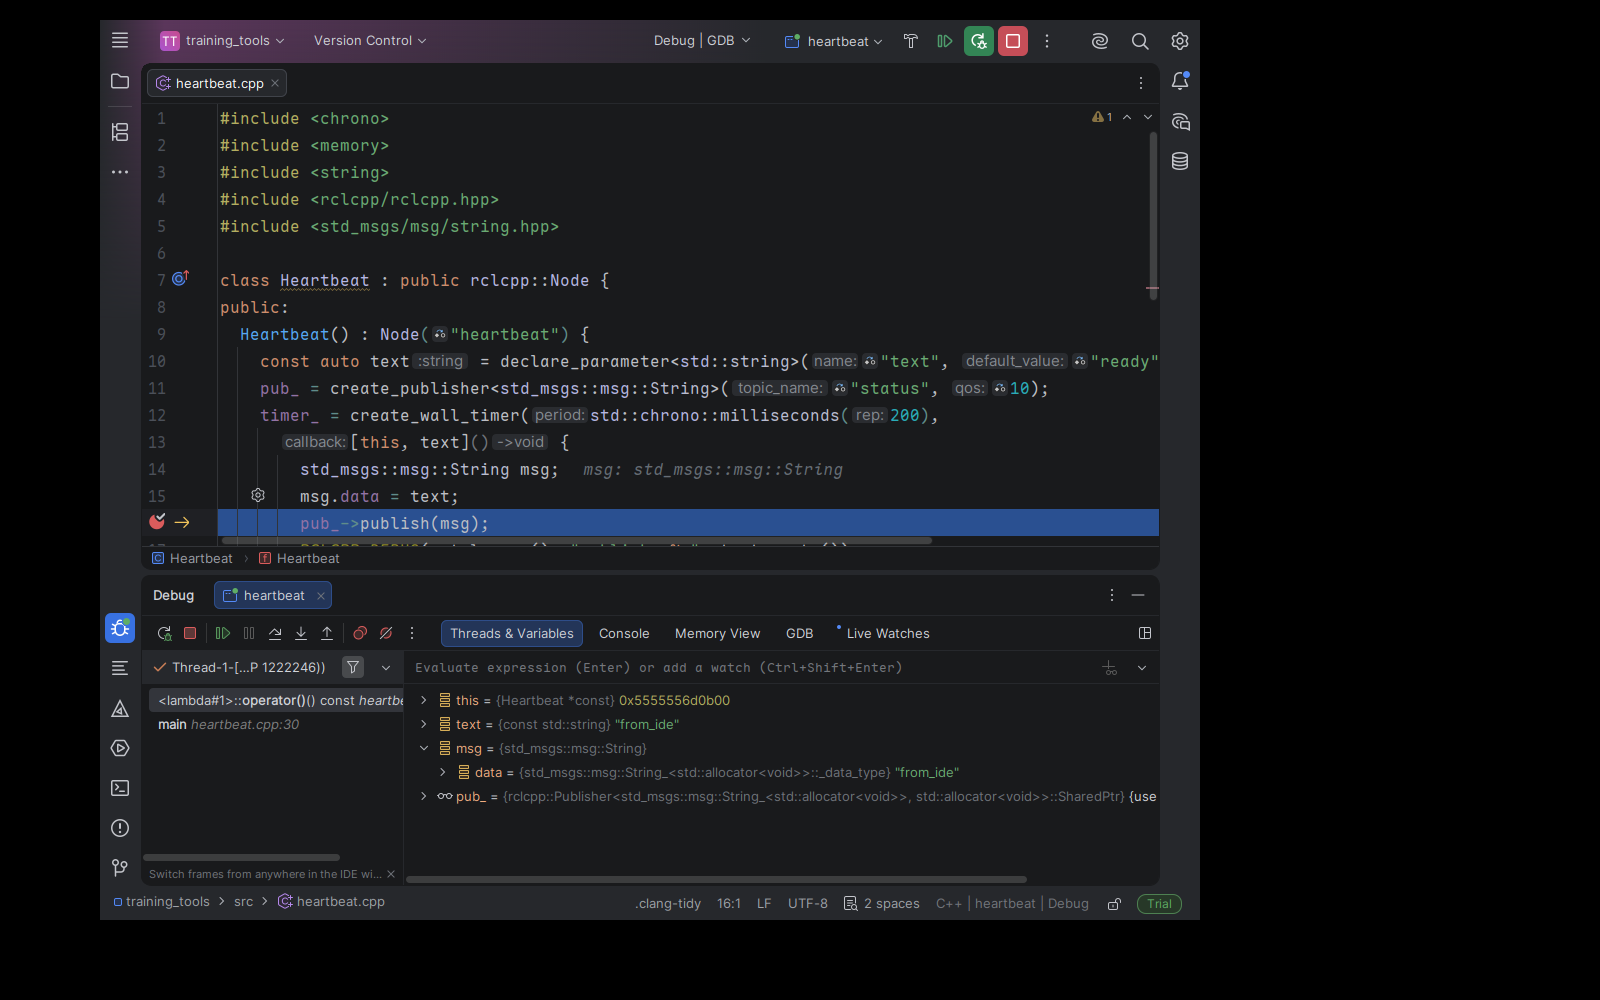
\includegraphics[width=0.9\textwidth,trim=100bp 180bp 400bp 300bp,clip]{images/ros2_clion_revised.png}
\caption{真实 CLion 调试窗口：发布回调暂停，消息文本已由运行参数覆盖}
\label{fig:ros2-clion-callback}
\end{figure}
\end{example}

CLion 的 Build 只负责所选构建目标。设置 \texttt{CMAKE\_INSTALL\_PREFIX} 仅改变安装目的地，不会自动执行安装。需要从 \texttt{ros2 run} 启动修改后的代码时，应由 colcon 重建并安装，或明确执行 IDE 的 install 目标；同时确认运行时加载的是该安装前缀。调试 IDE 构建目录中的目标时，则直接使用该目标。

\subsubsection{CLion：用编译数据库浏览多包工程}
编译数据库（compilation database）记录每个翻译单元实际使用的编译器、宏和头文件搜索路径，适合让 IDE 按 colcon 的真实参数索引代码。

\begin{example}[生成并核对索引来源]
\par\medskip\noindent\begin{minipage}{\linewidth}
\begin{tbash}
cd ~/ros2_ws
colcon build --packages-select training_tools --cmake-args -DCMAKE_EXPORT_COMPILE_COMMANDS=ON
test -f build/training_tools/compile_commands.json
\end{tbash}
\end{minipage}\par\smallskip
在 CLion 的 File $\rightarrow$ Open 中选择这个 JSON，再选 Open as Project，以编译数据库项目打开，核对 heartbeat.cpp 的包含路径。你可以在 \texttt{rclcpp/rclcpp.hpp} 上跳转到实际头文件，确认它来自当前发行版的安装目录。它只涵盖该包；修改项目根目录不会自动合并其他包的编译数据库。接口包须先构建，生成的消息头文件才存在。需要整个工作空间索引时，应显式收集各包的数据库并按工具支持方式合并。
\end{example}

\Needspace{18\baselineskip}
\subsubsection{CLion：排查库头文件的解析参数}
这时候你可能会碰到一个看起来很矛盾的情况：heartbeat.cpp 能编译，跳进 rclcpp.hpp 却满屏红线，提示它自己的子头文件找不到。先别急着重装 ROS，我们要检查的是编辑器解析这个文件时用了哪些参数。头文件通常没有独立的编译记录，编辑器需要借用包含它的源码的参数；如果这一步没有借到，只有系统头文件路径，就会找不到 ROS 的头文件。比较源码与外部头文件的 clangd 解析命令，确认缺少了哪些 include 路径。成功编译说明编译器的配置可用，不能顺便证明编辑器的配置也正确。

\begin{example}[给指定头文件补上当前源码的解析参数]
仅当你确认遇到了上面的参数缺失时再做这个例子。我们继续用同一个 training\_tools 工程，随书 \nolinkurl{examples/ros2/header_flags.py} 读取其编译数据库，输出一段 clangd 配置；它不执行编译命令，也不修改数据库。先把这个文件复制到 \texttt{\textasciitilde/ros2\_ws}，代码如下：
\Needspace{25\baselineskip}
\par\medskip\noindent\begin{minipage}{\linewidth}
\lstinputlisting[frame=single,basicstyle=\ttfamily\footnotesize,language=Python,numbers=left,firstline=1,lastline=22,caption={读取选定源码的编译命令}]{examples/ros2/header_flags.py}
\end{minipage}\par\smallskip
源码路径必须唯一对应一条命令，否则脚本会提示你核对路径或选对数据库。接下来只提取 include 路径、宏和语言标准，把相对 include 路径按原构建目录转成绝对路径；输出参数 \texttt{-o} 等构建选项没有复制过去。
\Needspace{26\baselineskip}
\par\medskip\noindent\begin{minipage}{\linewidth}
\lstinputlisting[frame=single,basicstyle=\ttfamily\footnotesize,language=Python,numbers=left,firstline=23,lastline=45,firstnumber=23,caption={生成只作用于指定头文件的配置}]{examples/ros2/header_flags.py}
\end{minipage}\par\smallskip
通用形式为 \texttt{python3 header\_flags.py 数据库 源码 头文件 [更多头文件]}。它输出 JSON，JSON 也是合法的 YAML。\texttt{If.PathMatch} 使用完整路径的正则表达式匹配，\texttt{re.escape} 把文件名中的点等字符转义，因此这段配置只作用于你选定的文件。先生成并查看片段：
\par\medskip\noindent\begin{minipage}{\linewidth}
\begin{tbash}
cd ~/ros2_ws
header=/opt/ros/$ROS_DISTRO/include/rclcpp/rclcpp/rclcpp.hpp
test -f "$header"
python3 header_flags.py build/training_tools/compile_commands.json \
  src/training_tools/src/heartbeat.cpp "$header" \
  > /tmp/ros-header-flags.json
cat /tmp/ros-header-flags.json
\end{tbash}
\end{minipage}\par\smallskip
这里的数据库和源码换成你的实际路径；头文件也以刚才跳转显示的路径为准。安装目录层级可能随软件包版本变化，先用 \texttt{test -f} 确认文件存在。确认输出与数据库中的 include 路径相符后，放进用户配置目录。已有配置先备份，再追加为一个新片段：
\par\medskip\noindent\begin{minipage}{\linewidth}
\begin{tbash}
cfg_dir="${XDG_CONFIG_HOME:-$HOME/.config}/clangd"
mkdir -p "$cfg_dir"
if [ -f "$cfg_dir/config.yaml" ]; then
  backup=$(mktemp "$cfg_dir/config.yaml.before-header-flags.XXXXXX")
  cp -p "$cfg_dir/config.yaml" "$backup"
  printf '备份：%s\n' "$backup"
  printf '\n---\n' >> "$cfg_dir/config.yaml"
fi
cat /tmp/ros-header-flags.json >> "$cfg_dir/config.yaml"
\end{tbash}
\end{minipage}\par\smallskip
配置放在这里，是因为库头文件位于工作空间之外，工作空间中的 \texttt{.clangd} 不会作用于它。IDE 需要使用同一个 \texttt{XDG\_CONFIG\_HOME}，默认不用额外设置；如果你用临时配置启动 IDE，就在那套临时目录里操作。随后关闭这个头文件标签，再从源码重新跳转，查看 Problems 中的诊断和实际解析参数。应能看到缺少的路径被补上，相应的找不到子头文件错误消失；保留诊断，并比较停用、恢复片段后的结果。

这只是把选定源码的解析条件借给选定头文件。其他包可能有不同的宏和路径，你要选它实际使用的源码重新生成；同一个头文件有多个编译上下文时也要先选定上下文。数据库、依赖或发行版变化后重新核对片段，不要把旧路径永久挂着。若仍有其他诊断，按其具体原因继续检查，不能一股脑关掉红线。
\end{example}

\begin{note}
可以从 Find Action 搜索 Show Clangd Tool Window 查看诊断工具；需要解析命令时，搜索 Registry，把 \texttt{clion.clang.clangd.debug} 临时设为 2，关闭并重开头文件后在 IDE 日志中查看 ASTWorker 的 command，查完恢复为 0。据此比较源码与头文件的实际 include 路径。配置格式和头文件参数借用机制分别见 \href{https://clangd.llvm.org/config}{clangd 配置文档}与 \href{https://clangd.llvm.org/design/compile-commands}{编译命令说明}；不要把 clangd 进程自身的参数与它解析某个文件的编译参数混在一起。
\end{note}

\begin{exercise}
\label{ex:v2-ros-header-context}
从 heartbeat.cpp 的数据库条目中找出 rclcpp 的 include 路径，说明它与 \texttt{rclcpp/rclcpp.hpp} 拼接后怎样定位文件。生成只匹配该头文件的配置，核对路径与宏；把源码参数换成不存在的路径，确认脚本会拒绝输出。若你的 IDE 确实存在上述缺失参数的问题，再在保留诊断的前提下比较启用片段前后的结果；没有此问题时记录实际参数，不必人为制造红线。
\end{exercise}

\begin{conclusion}
\begin{itemize}
\item 找不到 ament：检查 IDE 环境；找不到生成接口头：先构建接口包。
\item CLion 与 colcon 使用不同构建目录，避免 CMake 缓存和生成器相互覆盖；两者不必强制使用同一种生成器。
\item 断点不命中：检查 Debug 配置、正在运行的二进制路径，以及代码是否重新构建。
\item 源码能编译但外部头文件报错：比较二者实际解析参数；给指定头文件补参数后仍保留诊断，按具体错误继续查。
\item build、install、log、\texttt{.idea}、\texttt{cmake-build-*} 和生成的编译数据库通常不提交 Git；源码、清单和启动配置需要提交。
\end{itemize}
\end{conclusion}
\begin{exercise}
\label{ex:v2-ros-ide}
先停止上面的节点，清除运行配置中的 \texttt{-p text:=from\_ide} 等文本覆盖，再在 IDE 中把默认文本改为 \texttt{from\_debug} 并构建；依次从 IDE 和旧安装目录运行，每次观察后停止当前发布者，避免混在一起。解释为何可能看到不同文本，给出让 \texttt{ros2 run} 使用新代码的步骤。
\end{exercise}
